\documentclass[tikz,border=10pt]{standalone}
\usepackage[utf8]{inputenc}
\usepackage[T1]{fontenc}
\usepackage{lmodern}
\usepackage{xcolor}

\usetikzlibrary{arrows.meta, positioning, calc}

\definecolor{colText}{HTML}{222222}
\definecolor{colInput}{HTML}{DCEBFF}
\definecolor{colTemplate}{HTML}{EEF5FF}
\definecolor{colRoberta}{HTML}{E8E0FF}
\definecolor{colEmo}{HTML}{00A6C8}
\definecolor{colMode}{HTML}{7A3E9D}
\definecolor{colType}{HTML}{E28A00}
\definecolor{colCat}{HTML}{D64545}
\definecolor{cellFace}{HTML}{F2F2F2}
\definecolor{cellEdge}{HTML}{BBBBBB}

\begin{document}

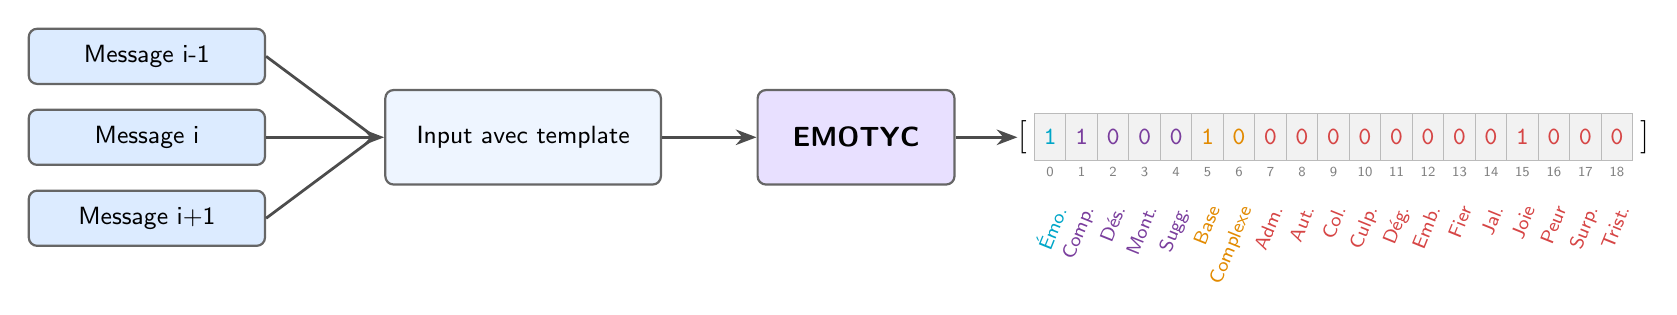
\begin{tikzpicture}[
    node distance=1cm,
    >=Stealth,
    basebox/.style={
        rectangle, rounded corners=3pt, draw=black!60,
        line width=0.8pt, align=center, font=\sffamily
    },
    msgbox/.style={basebox, fill=colInput, minimum width=3cm,
        minimum height=0.7cm, font=\sffamily\small},
    tempbox/.style={basebox, fill=colTemplate, minimum width=3.5cm,
        minimum height=1.2cm, font=\sffamily\small},
    modelbox/.style={basebox, fill=colRoberta, minimum width=2.5cm,
        minimum height=1.2cm, font=\sffamily\bfseries},
    vectorcell/.style={
        rectangle, draw=cellEdge, fill=cellFace,
        minimum width=0.4cm, minimum height=0.6cm,
        font=\ttfamily\bfseries\small,
        inner sep=0pt
    },
    vectorindex/.style={
        font=\tiny\sffamily,
        color=gray,
        inner sep=0pt
    },
    vectorlabel/.style={
        rotate=68,
        anchor=north east,
        font=\scriptsize\sffamily,
        inner sep=0pt
    }
]

    % --- INPUT SECTION ---
    \node[msgbox] (msg2) {Message i};
    \node[msgbox, above=0.3cm of msg2] (msg1) {Message i-1};
    \node[msgbox, below=0.3cm of msg2] (msg3) {Message i+1};

    % --- TEMPLATE SECTION ---
    \node[tempbox, right=1.5cm of msg2] (template) {Input avec template};

    % --- MODEL SECTION ---
    \node[modelbox, right=1.2cm of template] (emotyc) {EMOTYC};

    % --- ARROWS input -> template -> model ---
    \coordinate (sideInputPoint) at ($(template.west) + (-0.12, 0)$);
    \draw[-, line width=1pt, color=black!70] (msg1.east) -- (sideInputPoint);
    \draw[->, line width=1pt, color=black!70] (msg2.east) -- (template.west);
    \draw[-, line width=1pt, color=black!70] (msg3.east) -- (sideInputPoint);
    \draw[->, line width=1pt, color=black!70] (template.east) -- (emotyc.west);

    % --- VECTOR CELLS ---
    % Place first cell to the right of emotyc, leaving room for "["
    \coordinate (vecStart) at ($(emotyc.east) + (1.2, 0)$);

    \foreach \idx/\val/\col/\lab in {
        0/1/colEmo/Émo.,
        1/1/colMode/Comp.,
        2/0/colMode/Dés.,
        3/0/colMode/Mont.,
        4/0/colMode/Sugg.,
        5/1/colType/Base,
        6/0/colType/Complexe,
        7/0/colCat/Adm.,
        8/0/colCat/Aut.,
        9/0/colCat/Col.,
        10/0/colCat/Culp.,
        11/0/colCat/Dég.,
        12/0/colCat/Emb.,
        13/0/colCat/Fier,
        14/0/colCat/Jal.,
        15/1/colCat/Joie,
        16/0/colCat/Peur,
        17/0/colCat/Surp.,
        18/0/colCat/Trist.
    } {
        \node[vectorcell] (cell\idx) at ($(vecStart) + (\idx*0.4, 0)$)
            {\textcolor{\col}{\val}};
        \node[below=2pt of cell\idx, vectorindex] {\idx};
        \node[below=15pt of cell\idx, vectorlabel, text=\col] {\lab};
    }

    % --- BRACKETS placed symmetrically around the vector ---
    % cell0 center = vecStart, half-width = 0.2cm  => left edge of cell0  = vecStart - 0.2
    % cell18 center = vecStart + 7.2, half-width = 0.2 => right edge cell18 = vecStart + 7.4
    % We put both brackets at the same distance d=0.15 from the respective edges

    \node[font=\large\bfseries, inner sep=0pt]  (lbracket)
        at ($(vecStart) + (-0.35, 0)$) {$[$};

    \node[font=\large\bfseries, inner sep=0pt]  (rbracket)
        at ($(vecStart) + (18*0.4 + 0.35, 0)$) {$]$};

    % Arrow from emotyc to left bracket
    \draw[->, line width=1pt, color=black!70]
        (emotyc.east) -- (lbracket.west);

\end{tikzpicture}
\end{document}
